\chapter{Advanced Control Techniques}



\section{Section 1: Feedforward \& Ratio Control [15M] [Priority: High]}

\subsection{1. Feedforward Control System}
A \textbf{feedforward control system} is an anticipatory control strategy where disturbances are measured and corrected for before they have a chance to affect the controlled process variable.

\begin{figure}[H]
\centering
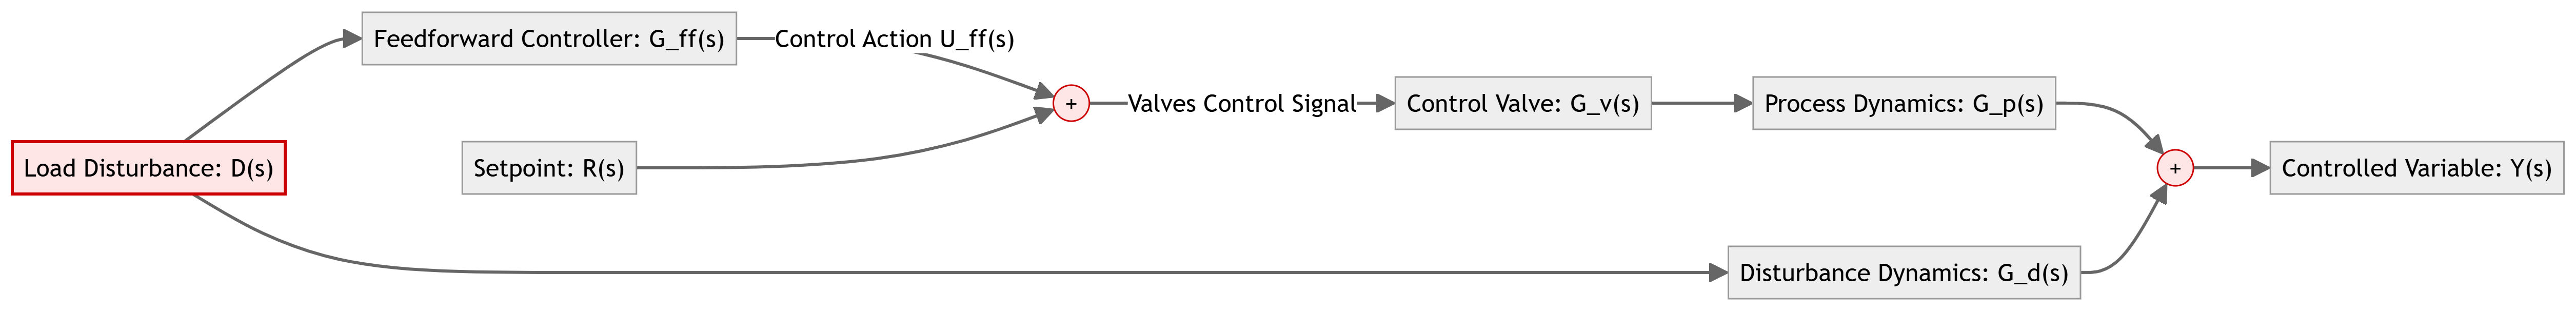
\includegraphics[width=0.75\textwidth,height=0.32\textheight,keepaspectratio]{../Images/chapter_04/feedforward_block.png}
\caption{Feedforward Control System Block Diagram}
\end{figure}

\subsubsection{A. Mathematical Derivation of Feedforward Controller}
Consider the block diagram of the process system. The controlled output $Y(s)$ is affected by both the control action $U(s)$ and the load disturbance $D(s)$:
\[ Y(s) = G_p(s) G_v(s) U(s) + G_d(s) D(s) \]
where:
\begin{itemize}
  \item $G_p(s)$: Process dynamics transfer function.
  \item $G_v(s)$: Control valve transfer function.
  \item $G_d(s)$: Disturbance dynamics transfer function.
\end{itemize}

The feedforward controller $G_{ff}(s)$ measures the disturbance $D(s)$ and generates the control signal $U_{ff}(s) = G_{ff}(s) D(s)$.
For perfect control, we want to maintain the output at zero deviation ($Y(s) = 0$) despite changes in $D(s)$:
\[ G_p(s) G_v(s) [G_{ff}(s) D(s)] + G_d(s) D(s) = 0 \]

Dividing by $D(s)$:
\[ G_p(s) G_v(s) G_{ff}(s) + G_d(s) = 0 \]

Solving for the ideal Feedforward Controller Transfer Function $G_{ff}(s)$:
\[ G_{ff}(s) = -\frac{G_d(s)}{G_v(s) G_p(s)} \]

\textit{(Note: The negative sign indicates that the controller must apply a corrective action in the opposite direction of the disturbance deflection).}

\subsubsection{B. Feedback vs. Feedforward Control Comparison}

\begin{table}[H]
\centering
\begin{tabular}{|p{\dimexpr 0.2\textwidth - 2\tabcolsep - 1.5\arrayrulewidth\relax}|p{\dimexpr 0.4\textwidth - 2\tabcolsep - 1.5\arrayrulewidth\relax}|p{\dimexpr 0.4\textwidth - 2\tabcolsep - 1.5\arrayrulewidth\relax}|}
\hline
Feature / Criteria & Feedback Control & Feedforward Control \\
\hline
\textbf{Operating Principle} & Reactive; acts only after a deviation in the output occurs. & Proactive; acts before a deviation in the output occurs. \\
\hline
\textbf{Measurement Parameter} & Measures the controlled variable ($Y(s)$). & Measures the load disturbance ($D(s)$). \\
\hline
\textbf{Stability} & Can cause instability and oscillations if tuned aggressively. & Inherently stable because it does not introduce a feedback loop. \\
\hline
\textbf{Process Knowledge} & Requires minimal process model knowledge. & Requires an accurate mathematical model of the process. \\
\hline
\textbf{Disturbance Rejection} & Rejects all disturbances, both known and unknown. & Rejects only the specific, measured disturbances. \\
\hline
\end{tabular}
\end{table}

\begin{figure}[H]
\centering
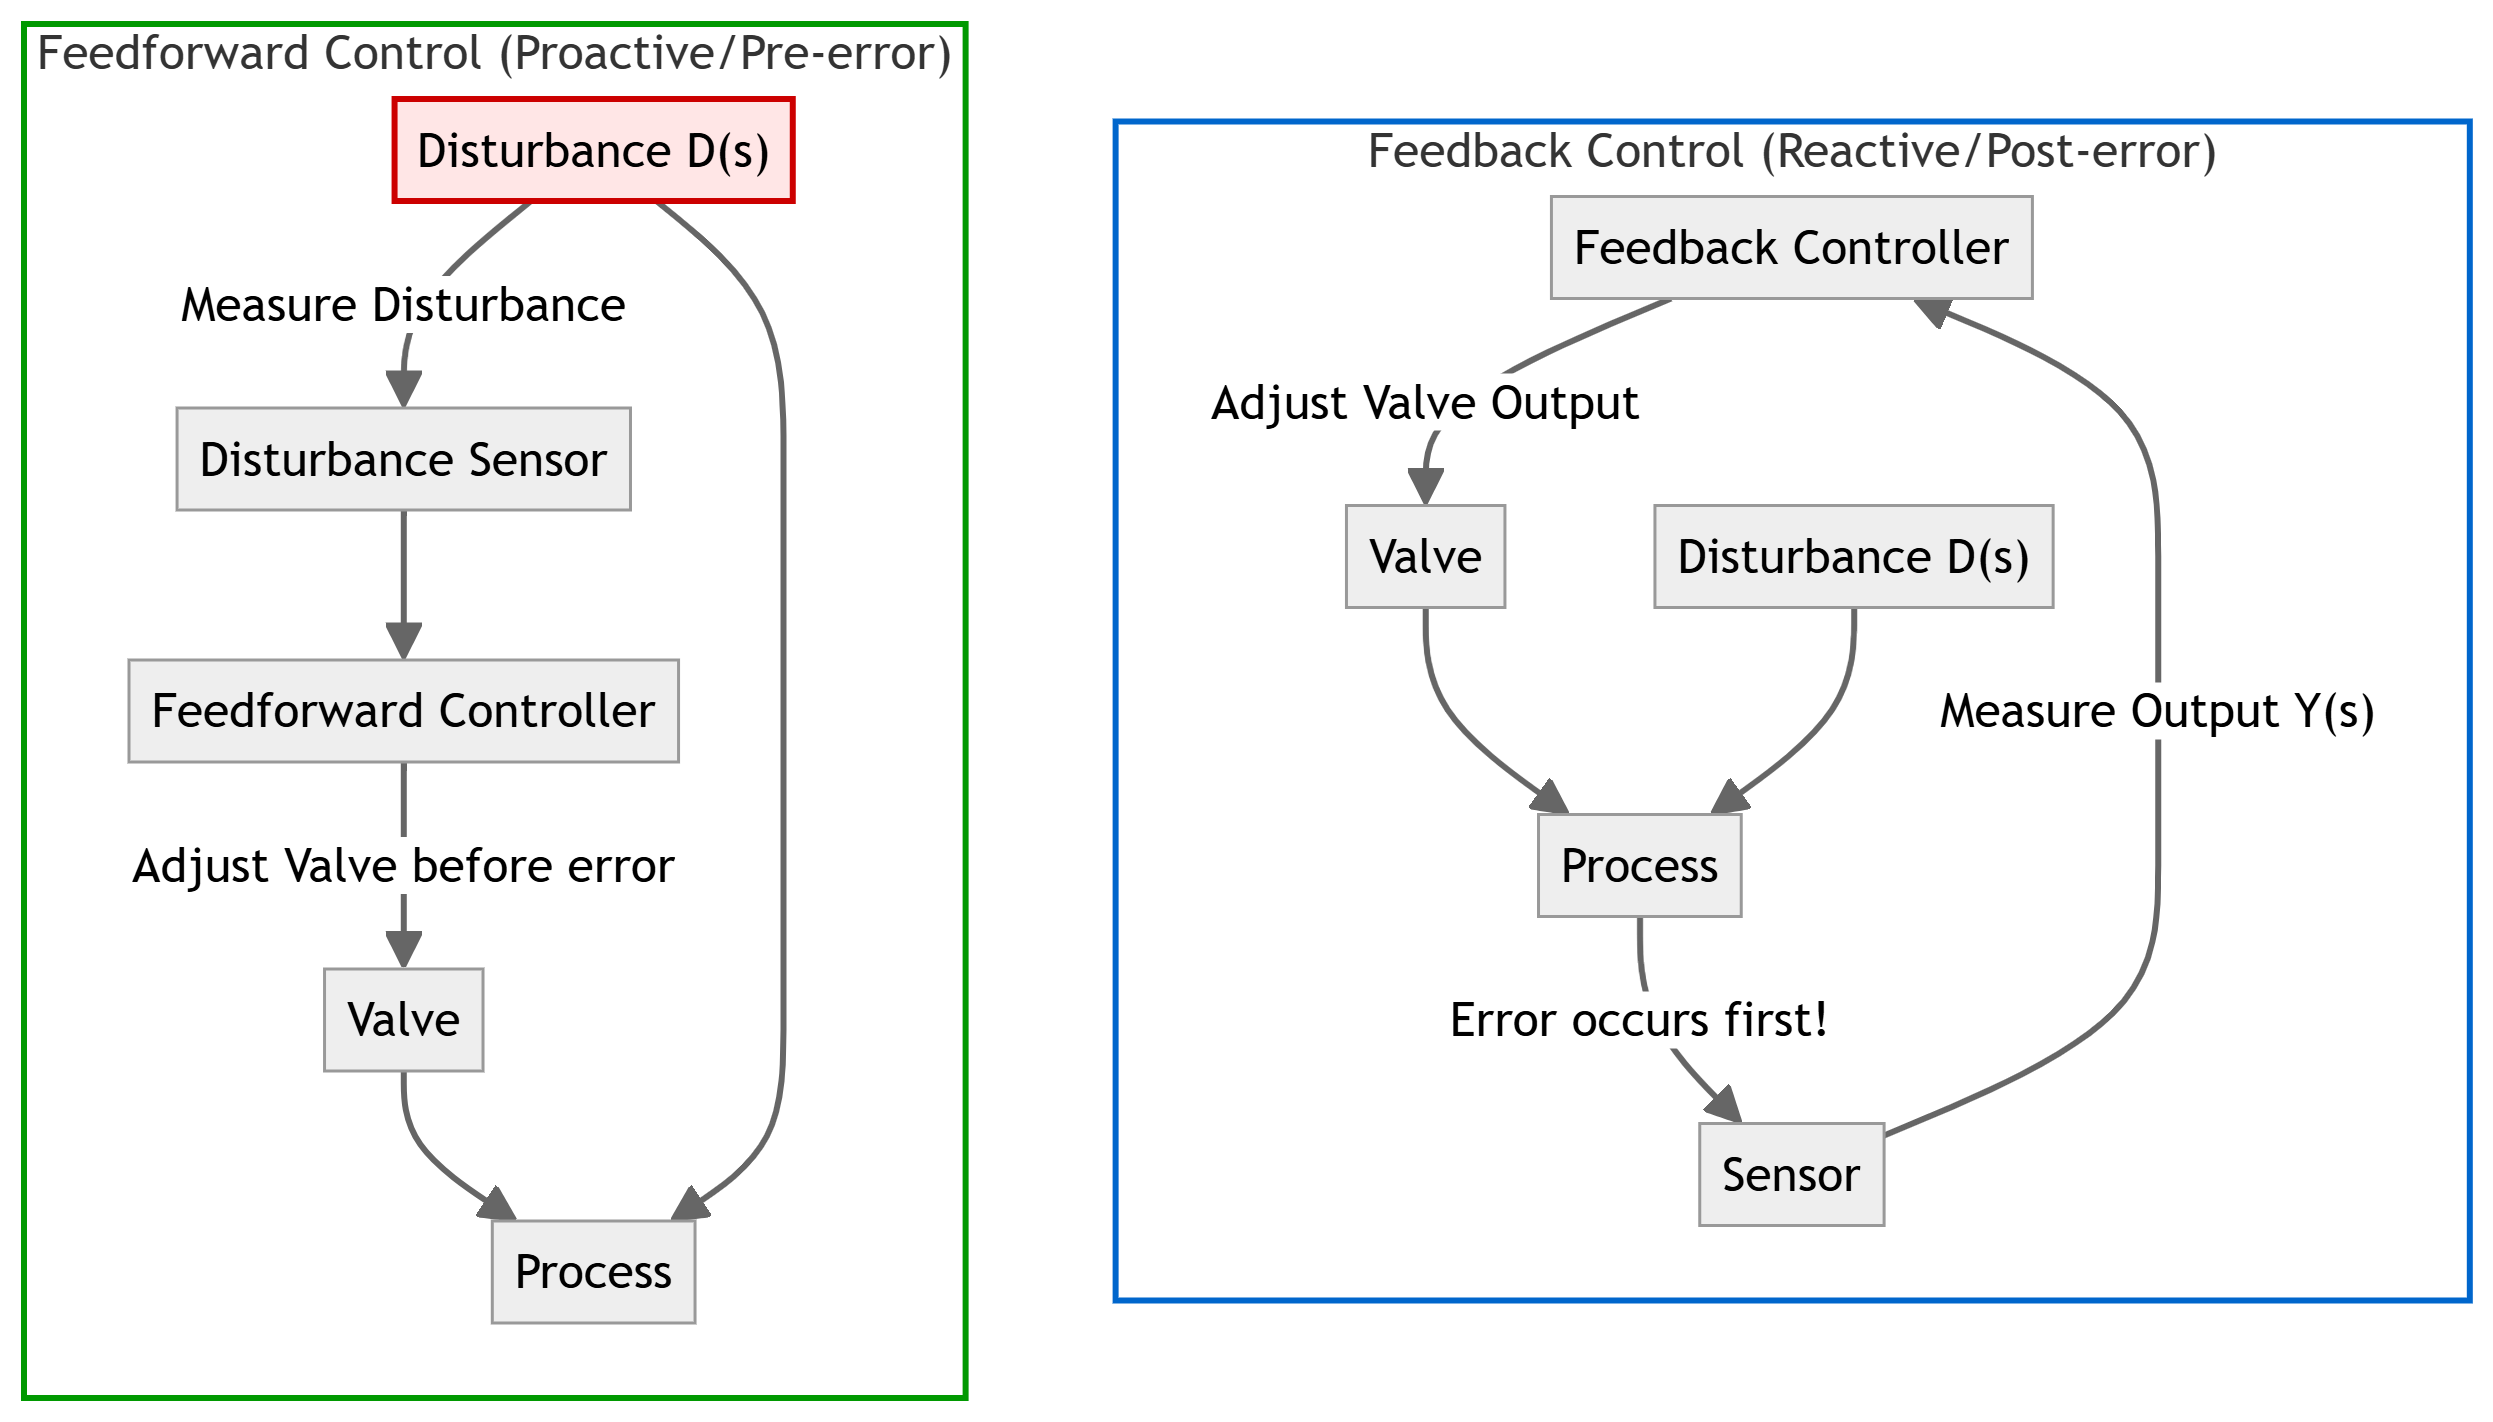
\includegraphics[width=0.75\textwidth,height=0.32\textheight,keepaspectratio]{../Images/chapter_04/feedback_vs_feedforward.png}
\caption{Feedback vs. Feedforward Control Loop Comparison}
\end{figure}

\subsubsection{C. Heat Exchanger Case Study}
In an industrial shell-and-tube heat exchanger, process fluid is heated by steam.
\begin{itemize}
  \item \textbf{Goal:} Maintain process fluid outlet temperature at setpoint.
  \item \textbf{Load Disturbances:} Inlet process fluid flow rate, inlet process fluid temperature, and steam pressure variations.
  \item \textbf{FF Control Action:} A sensor measures the inlet flow rate (disturbance). If the flow rate increases, the feedforward controller immediately opens the steam control valve to supply more heat before the outlet temperature has a chance to drop.
\end{itemize}


\subsection{2. Ratio Control System}
A \textbf{ratio control system} is a specialized feedforward control loop used to maintain a constant ratio between two process flow streams.

\subsubsection{A. Wild Flow vs. Controlled Flow}
\begin{itemize}
  \item \textbf{Wild Flow ($F_W$):} The primary stream flow rate. It is determined by upstream plant conditions and cannot be adjusted by the ratio controller.
  \item \textbf{Controlled Flow ($F_C$):} The secondary stream flow rate. Its control valve is adjusted by the controller to maintain the desired ratio:
\end{itemize}
  \[ R = \frac{F_C}{F_W} \]

\subsubsection{B. Multiplier vs. Divider Schemes}
\begin{itemize}
  \item \textbf{Multiplier Scheme (Recommended):}
\end{itemize}
  The wild flow $F_W$ is measured and multiplied by the desired ratio $R$ to calculate the setpoint for the controlled flow loop ($F_C^* = R \times F_W$).
\begin{itemize}
  \item \textbf{Divider Scheme:}
\end{itemize}
  Both flows are measured, and their ratio is calculated ($R_{act} = F_C / F_W$) and compared to the setpoint ratio $R$.
\begin{itemize}
  \item \textit{Disadvantage:} If the wild flow drops to zero ($F_W = 0$), the division results in a divide-by-zero error, causing controller saturation and loop instability. Therefore, the \textbf{multiplier scheme} is preferred.
\end{itemize}

\begin{figure}[H]
\centering
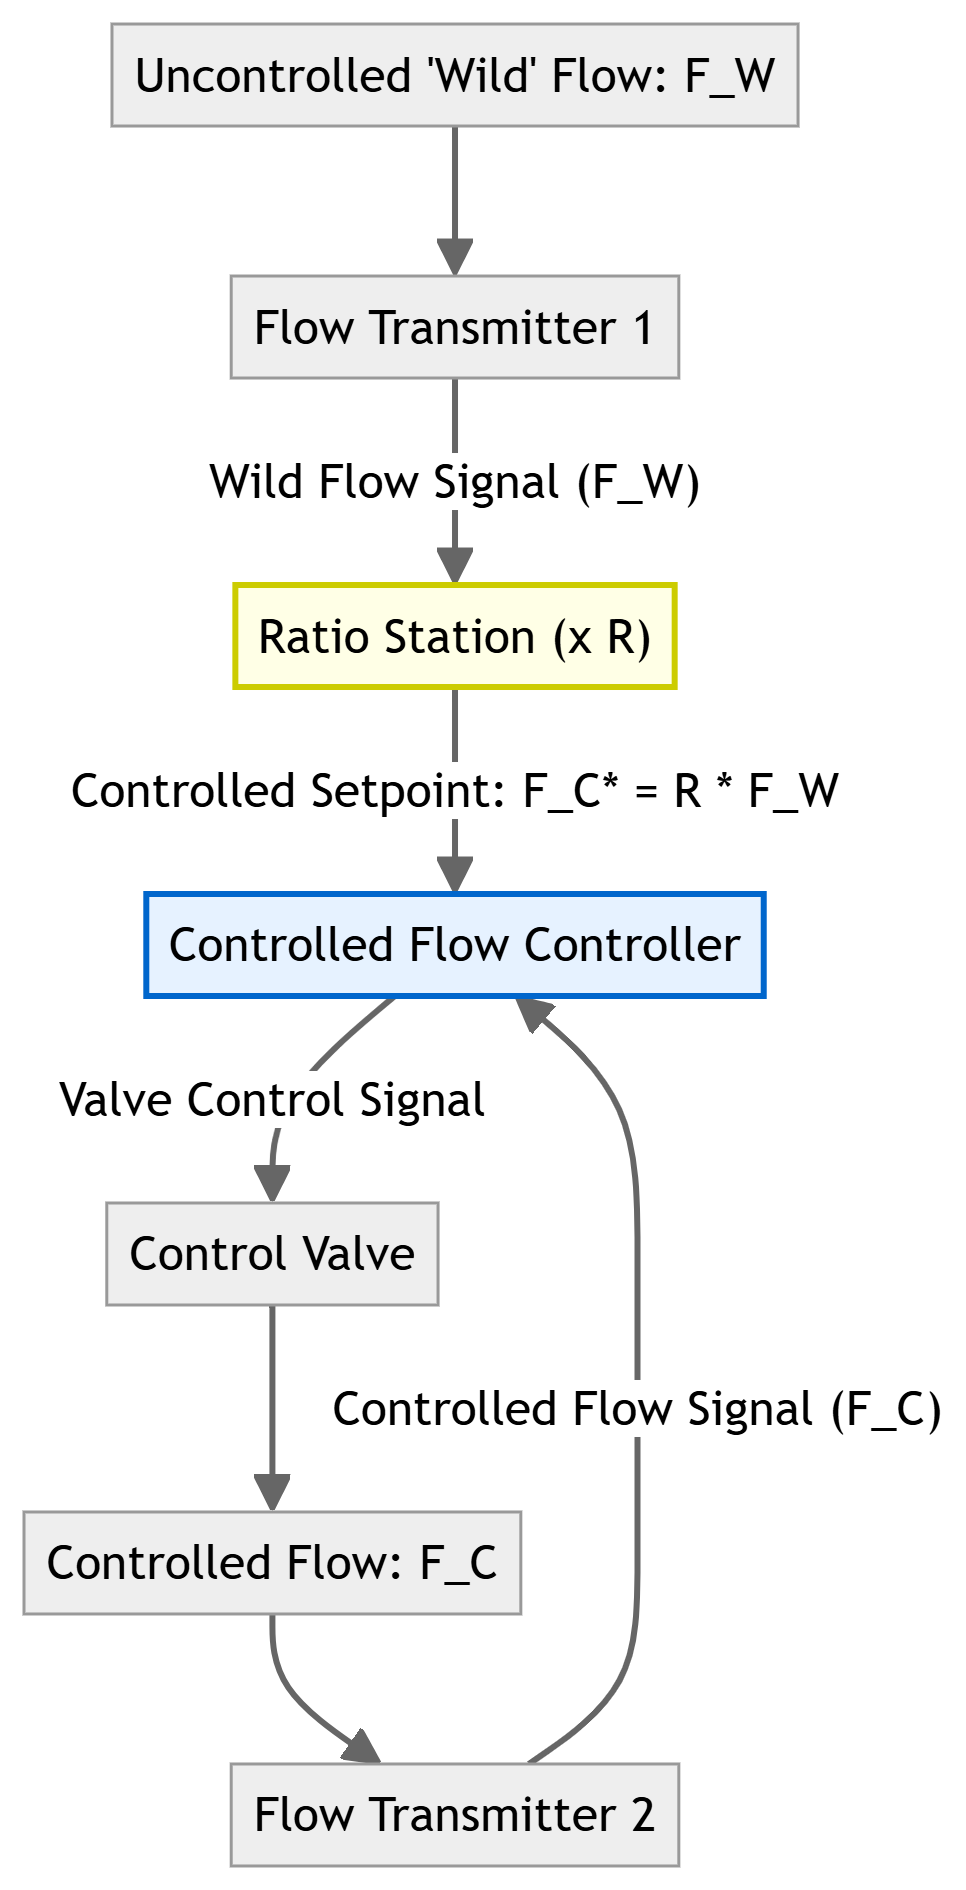
\includegraphics[width=0.75\textwidth,height=0.32\textheight,keepaspectratio]{../Images/chapter_04/ratio_control.png}
\caption{Ratio Control System (Multiplier Scheme)}
\end{figure}

\begin{itemize}
  \item \textbf{Application Example:}
  \item \textit{Fuel-Air Ratio Control:} Maintaining the exact stoichiometric ratio of air and fuel entering a combustion furnace to ensure efficient combustion and reduce emissions.
\end{itemize}


\section{Section 2: Cascade Control System [15M] [Priority: High]}

\subsection{1. Definition and Operating Principle}
A \textbf{cascade control system} consists of two nested feedback loops: a \textbf{primary (outer) loop} and a \textbf{secondary (inner) loop}. The primary controller (Master) monitors the main controlled variable and calculates a control output, which serves as the setpoint for the secondary controller (Slave). The slave controller directly adjusts the final control valve.

\begin{figure}[H]
\centering
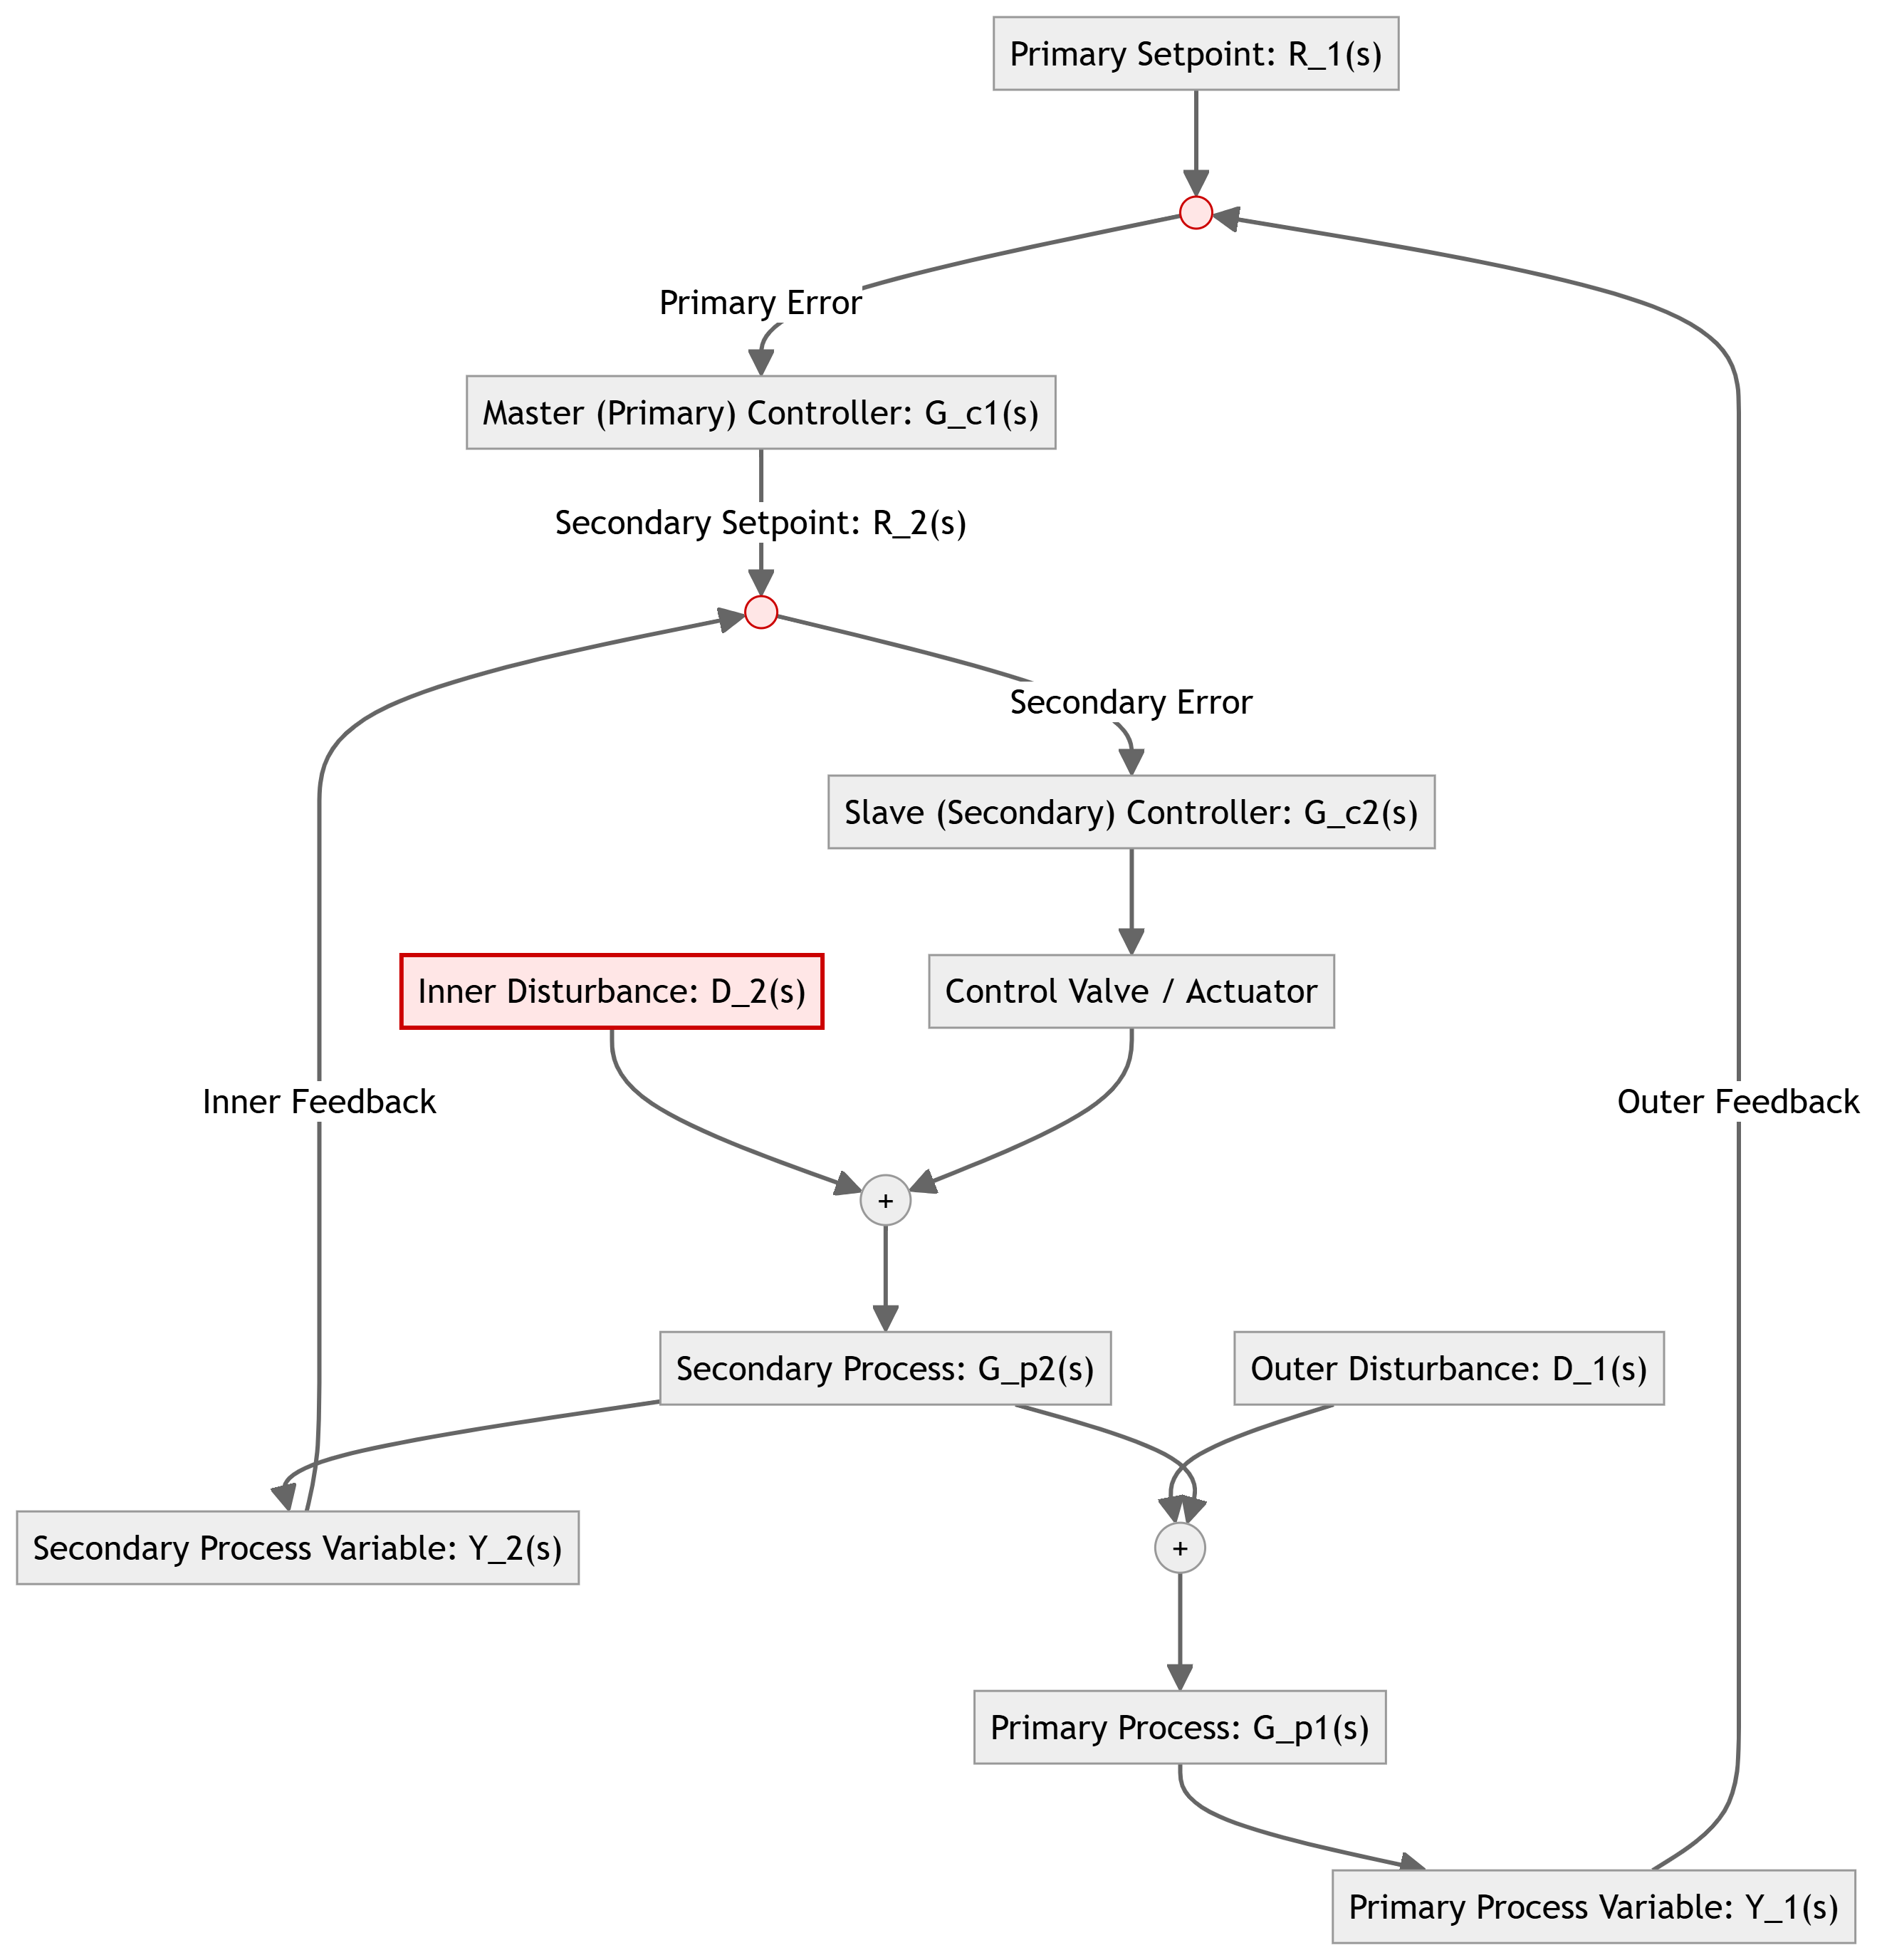
\includegraphics[width=0.75\textwidth,height=0.32\textheight,keepaspectratio]{../Images/chapter_04/cascade_block.png}
\caption{Cascade Control Loop Block Diagram}
\end{figure}

\subsubsection{Operating Principle:}
\begin{itemize}
  \item \textbf{Inner (Slave) Loop:} Deployed close to the source of the disturbance (e.g., fuel header pressure). It is designed to be fast-acting.
  \item \textbf{Outer (Master) Loop:} Monitors the primary slow process variable (e.g., furnace temperature). It calculates the setpoint for the inner loop.
  \item If a pressure spike occurs in the fuel line, the slave loop detects the change and corrects the valve position immediately, before the primary process temperature is affected.
\end{itemize}


\subsection{2. Advantages of Cascade Control}
\begin{itemize}
  \item \textbf{Fast Disturbance Rejection:} Rejects secondary disturbances within the inner loop before they can propagate and affect the primary process variable.
  \item \textbf{Reduced Phase Lag:} Breaking a multi-capacity process into two smaller loops reduces the overall phase lag, allowing higher controller gains and faster response.
  \item \textbf{Linearization:} The inner loop linearizes the valve characteristics and compensates for actuator non-linearities like hysteresis and stiction.
\end{itemize}


\section{Section 3: Special Loop Architectures (Split-Range \& Override) [15M] [Priority: High]}


\subsection{1. Split-Range (Duplex) Control}
\textbf{Split-range control} is a loop configuration where a single controller output (CO) is split to control two or more final control elements (valves) acting in sequence.

\begin{figure}[H]
\centering
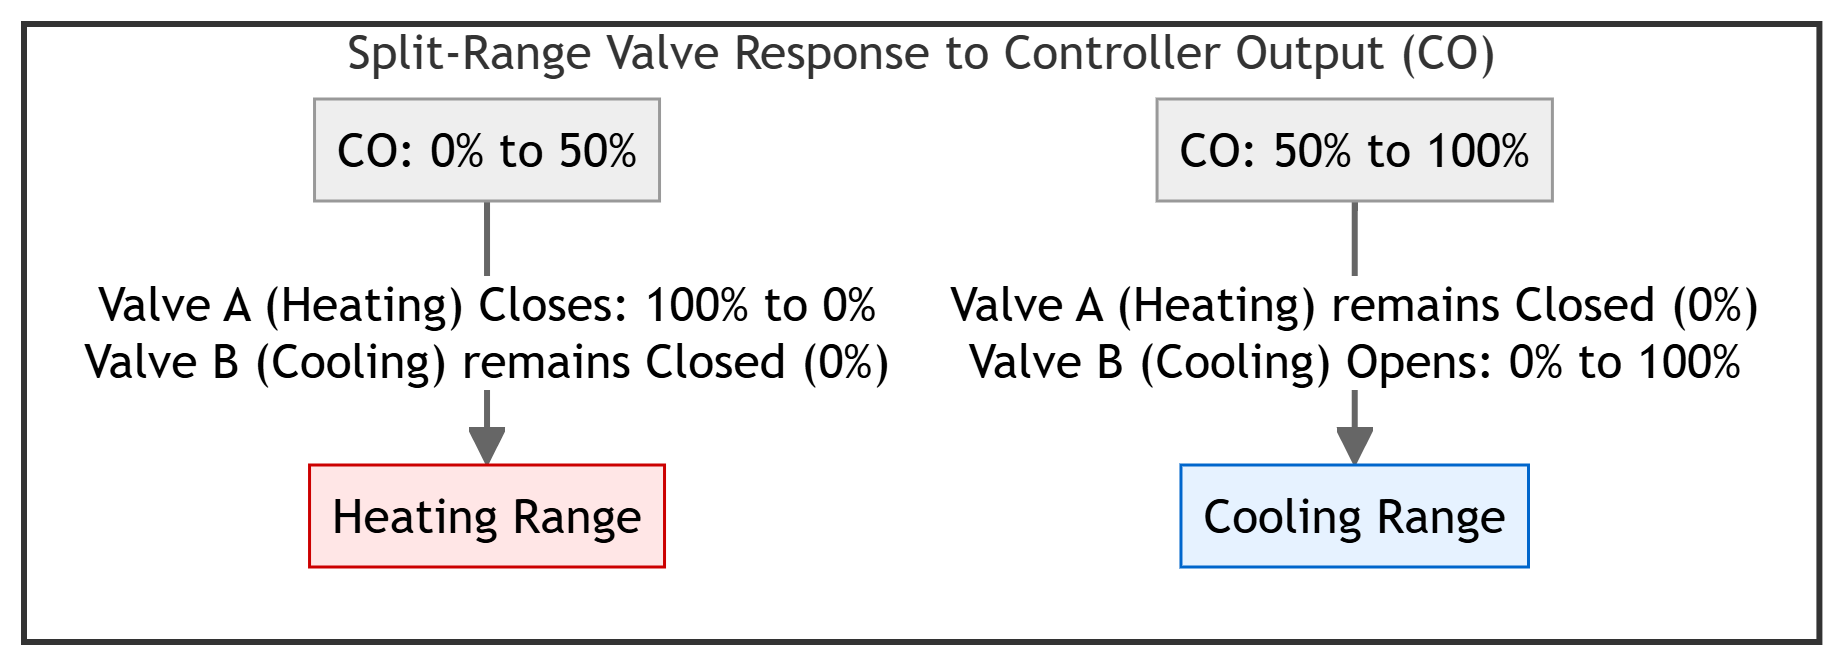
\includegraphics[width=0.75\textwidth,height=0.32\textheight,keepaspectratio]{../Images/chapter_04/split_range.png}
\caption{Split-Range (Duplex) Control Loop Graph}
\end{figure}

\subsubsection{A. Working Principle}
The controller output range ($0\text{--}100\%$) is split into sub-ranges for each valve:
\begin{itemize}
  \item \textbf{Valve A (Heating Valve - Air-to-Open):}
  \item At $0\%$ CO: Fully Open ($3\ \text{psi}$ signal).
  \item At $50\%$ CO: Fully Closed ($9\ \text{psi}$ signal).
  \item At $50\text{--}100\%$ CO: Remains Closed.
  \item \textbf{Valve B (Cooling Valve - Air-to-Close):}
  \item At $0\text{--}50\%$ CO: Remains Closed ($9\ \text{psi}$ signal).
  \item At $50\%$ CO: Fully Closed.
  \item At $100\%$ CO: Fully Open ($15\ \text{psi}$ signal).
\end{itemize}

\subsubsection{B. Industrial Example}
\begin{itemize}
  \item \textbf{Chemical Jacketed Reactor:}
\end{itemize}
  To control reactor temperature, a single PID controller adjusts both steam (heating) and cooling water (cooling) valves. From $0\text{--}50\%$ CO, the steam valve closes. From $50\text{--}100\%$ CO, the cooling valve opens. This ensures both valves are never open at the same time, preventing energy waste.


\subsection{2. Override (Selective) Control}
\textbf{Override (selective) control} is a protective control strategy where two or more controllers share a single control valve through a selector block (High Selector or Low Selector).

\begin{figure}[H]
\centering
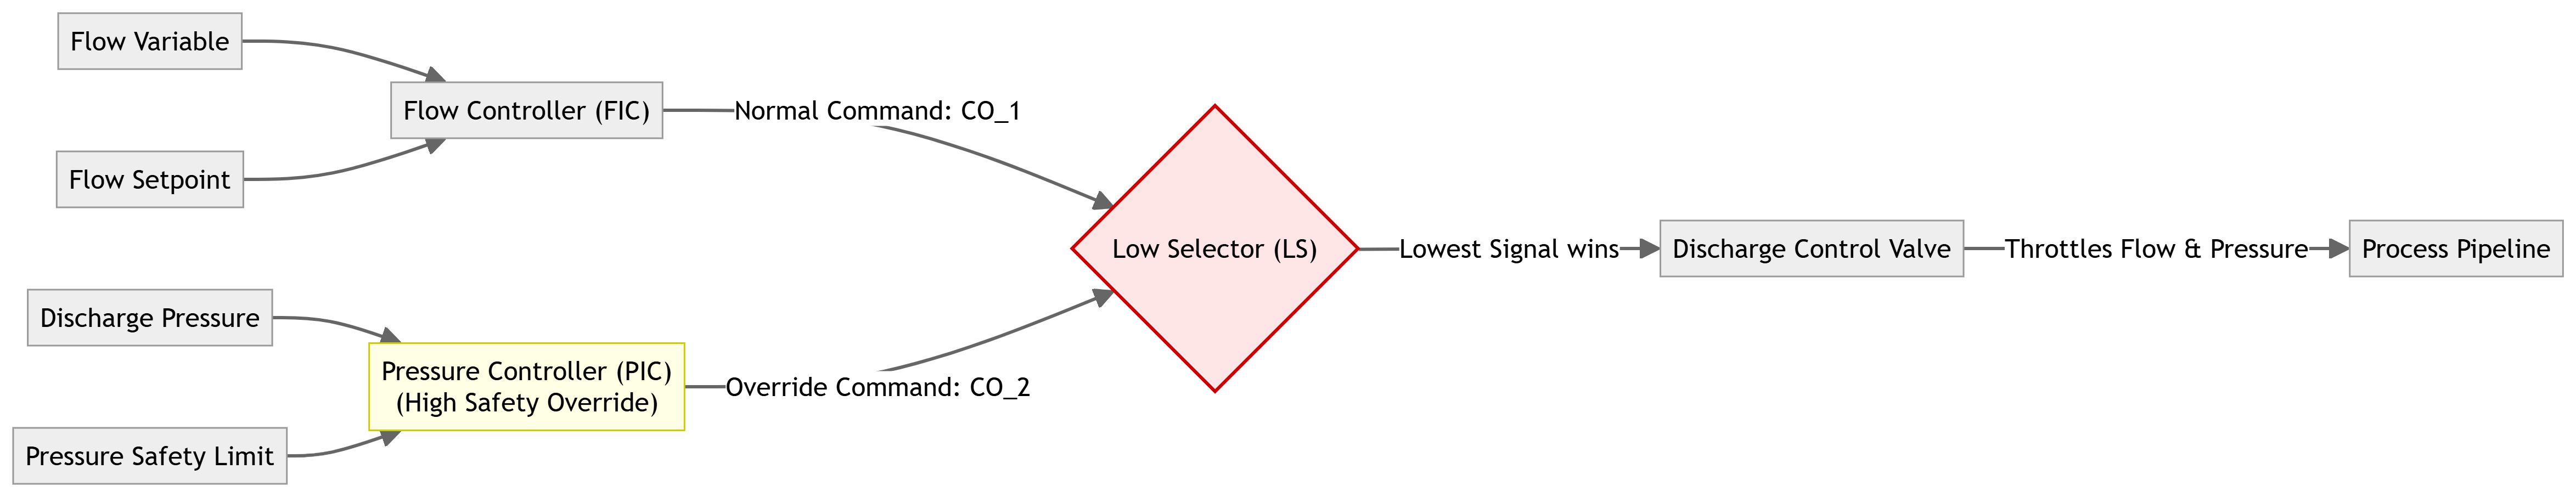
\includegraphics[width=0.75\textwidth,height=0.32\textheight,keepaspectratio]{../Images/chapter_04/override_control.png}
\caption{Override (Selective) Control Loop}
\end{figure}

\subsubsection{A. Working Principle \& Safety Protection}
\begin{itemize}
  \item Under normal operating conditions, the primary controller (e.g., Flow Controller) maintains the process variable at the setpoint.
  \item If a secondary variable (e.g., discharge pressure or motor current) exceeds a safety threshold, the safety override controller activates.
  \item The \textbf{Low Selector (LS)} or \textbf{High Selector (HS)} compares the controller outputs and routes the safer signal to the valve:
  \item \textit{Low Selector:} Passes the lowest controller output. Used to limit high pressures or flows.
  \item \textit{High Selector:} Passes the highest controller output. Used to maintain minimum flow to prevent pump damage.
\end{itemize}

\subsubsection{B. Necessity}
\begin{itemize}
  \item Prevents equipment damage (e.g., pipeline overpressure or pump cavitation).
  \item Avoids plant shutdowns by temporarily throttling the process instead of tripping the system.
\end{itemize}


\section{Section 4: Advanced Adaptive \& Model-Based Control [15M] [Priority: High]}


\subsection{1. Adaptive Control}
An \textbf{adaptive controller} automatically adjusts its tuning gains ($K_c, \tau_I, \tau_D$) in real-time to compensate for changes in process dynamics, non-linearities, or environmental conditions.

\begin{table}[H]
\centering
\begin{tabular}{|p{\dimexpr 0.2\textwidth - 2\tabcolsep - 1.5\arrayrulewidth\relax}|p{\dimexpr 0.4\textwidth - 2\tabcolsep - 1.5\arrayrulewidth\relax}|p{\dimexpr 0.4\textwidth - 2\tabcolsep - 1.5\arrayrulewidth\relax}|}
\hline
Feature / Criteria & Model Reference Adaptive Control (MRAC) & Self-Tuning Regulators (STR) \\
\hline
\textbf{Operating Loop} & Uses an explicit reference model in parallel. & Identifies process parameters online using recursive estimation. \\
\hline
\textbf{Parameter Update} & Updates controller parameters based on model tracking error. & Updates controller parameters by solving design equations. \\
\hline
\textbf{Complexity} & Simpler calculation loop; relies on direct gradient rules. & Highly complex; requires online parameter estimation. \\
\hline
\textbf{Response Speed} & Fast adaptation to transient path deviations. & Slower adaptation due to parameter identification lag. \\
\hline
\end{tabular}
\end{table}

\subsubsection{A. Model Reference Adaptive Control (MRAC)}
An ideal reference model defines the desired response of the closed-loop system to a setpoint change. The adjustment mechanism compares the actual process output ($Y$) with the model output ($Y_m$) and updates the controller gains using adaptation algorithms (e.g., MIT rule) to drive the error to zero.

\begin{figure}[H]
\centering
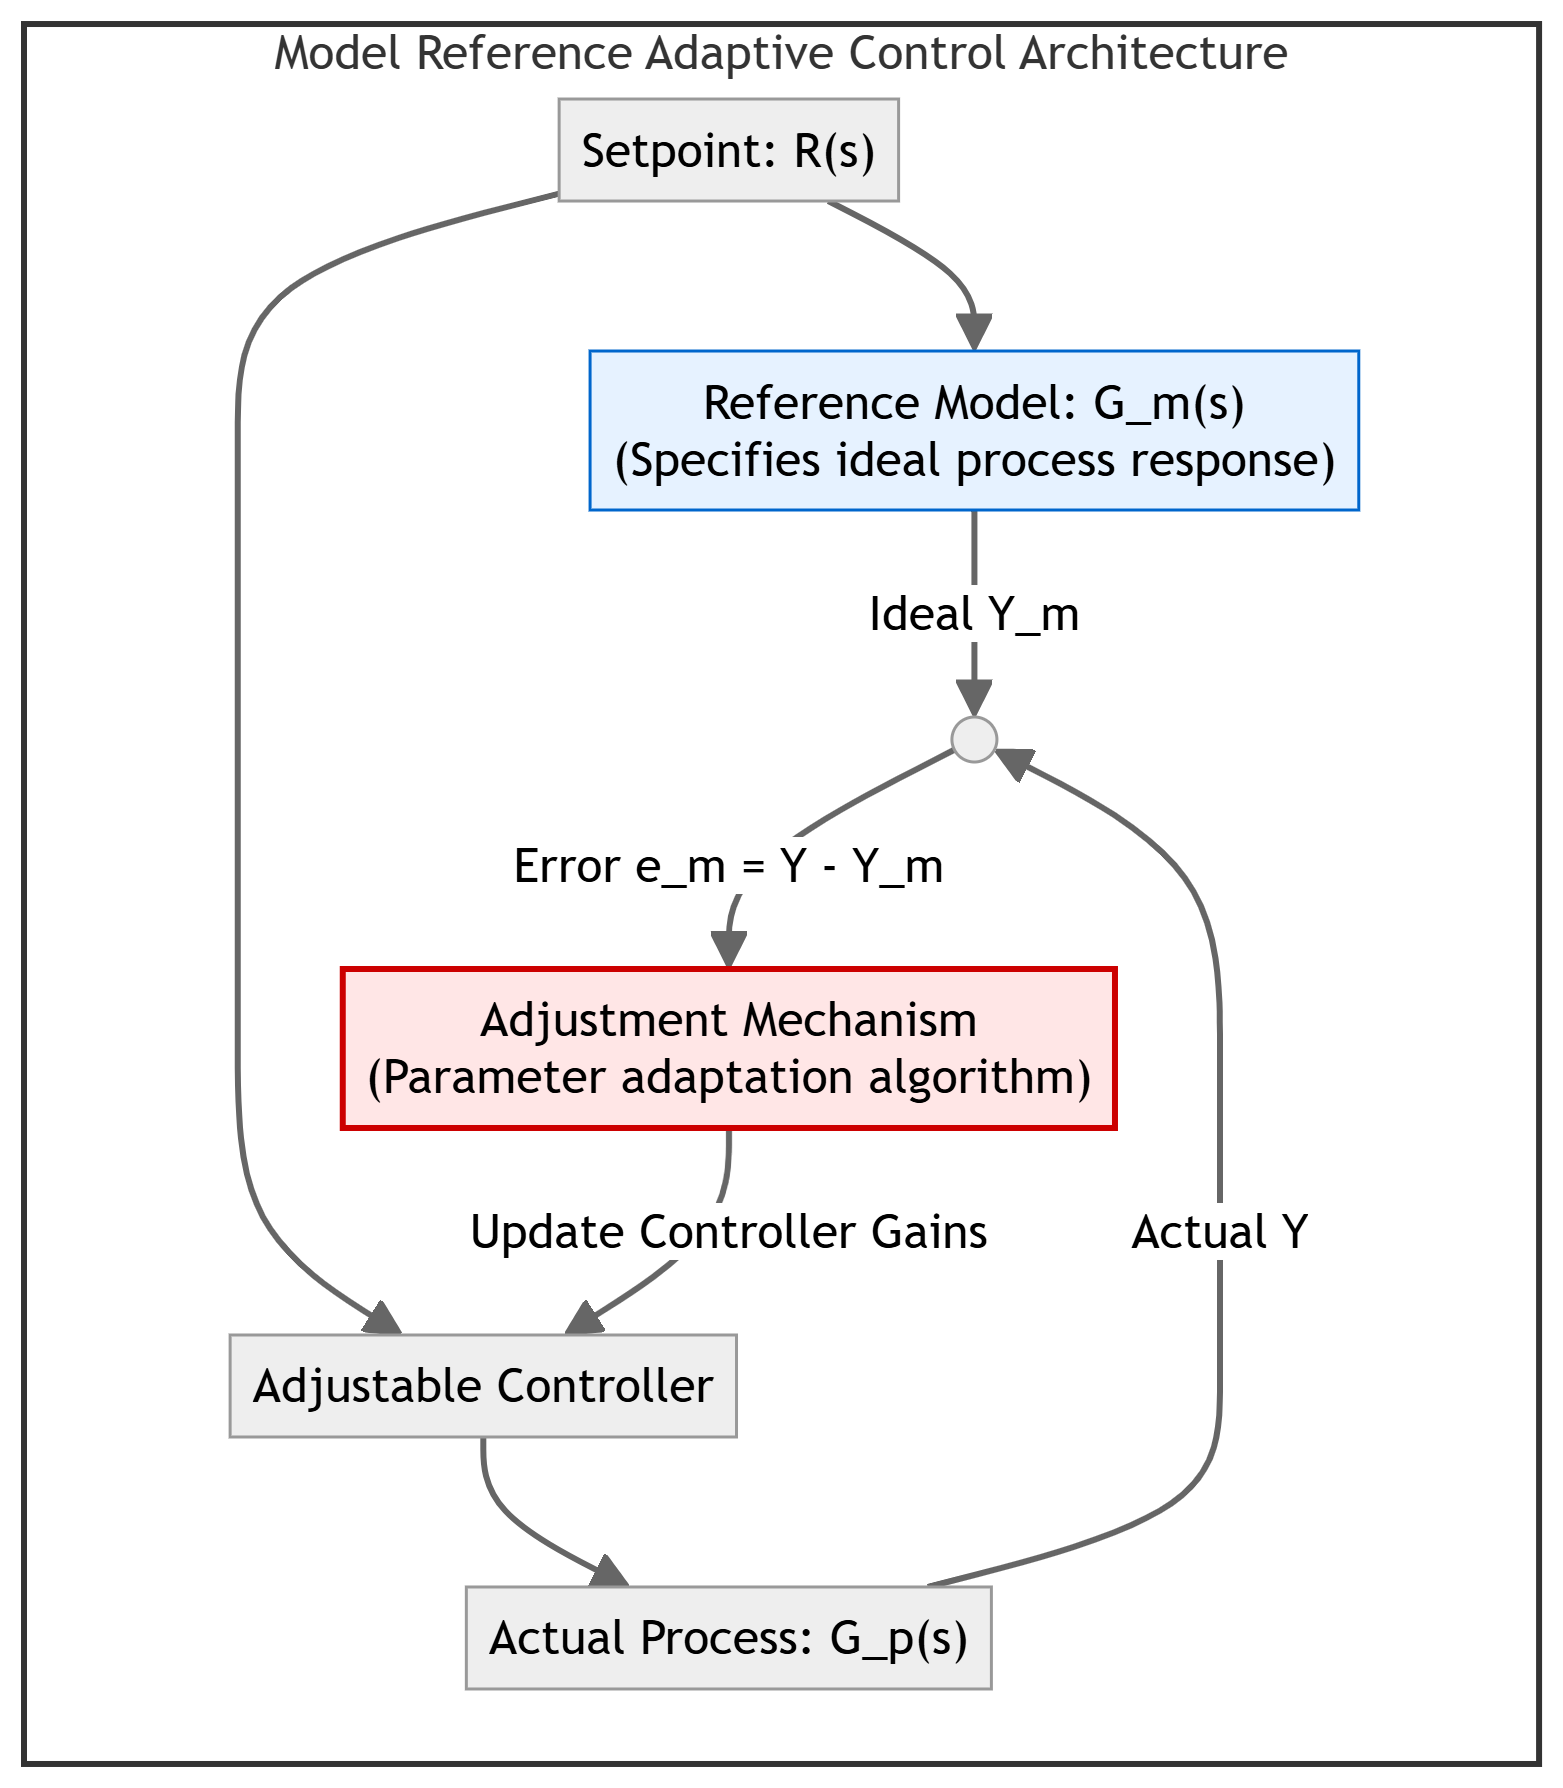
\includegraphics[width=0.75\textwidth,height=0.32\textheight,keepaspectratio]{../Images/chapter_04/mrac_block.png}
\caption{Model Reference Adaptive Control (MRAC)}
\end{figure}

\subsubsection{B. Self-Tuning Regulators (STR)}
An STR contains an online parameter estimator that continuously identifies the process parameters (e.g., using Recursive Least Squares - RLS). A controller design block uses these estimated parameters to calculate new controller gains (e.g., using pole placement) and updates the controller.

\begin{figure}[H]
\centering
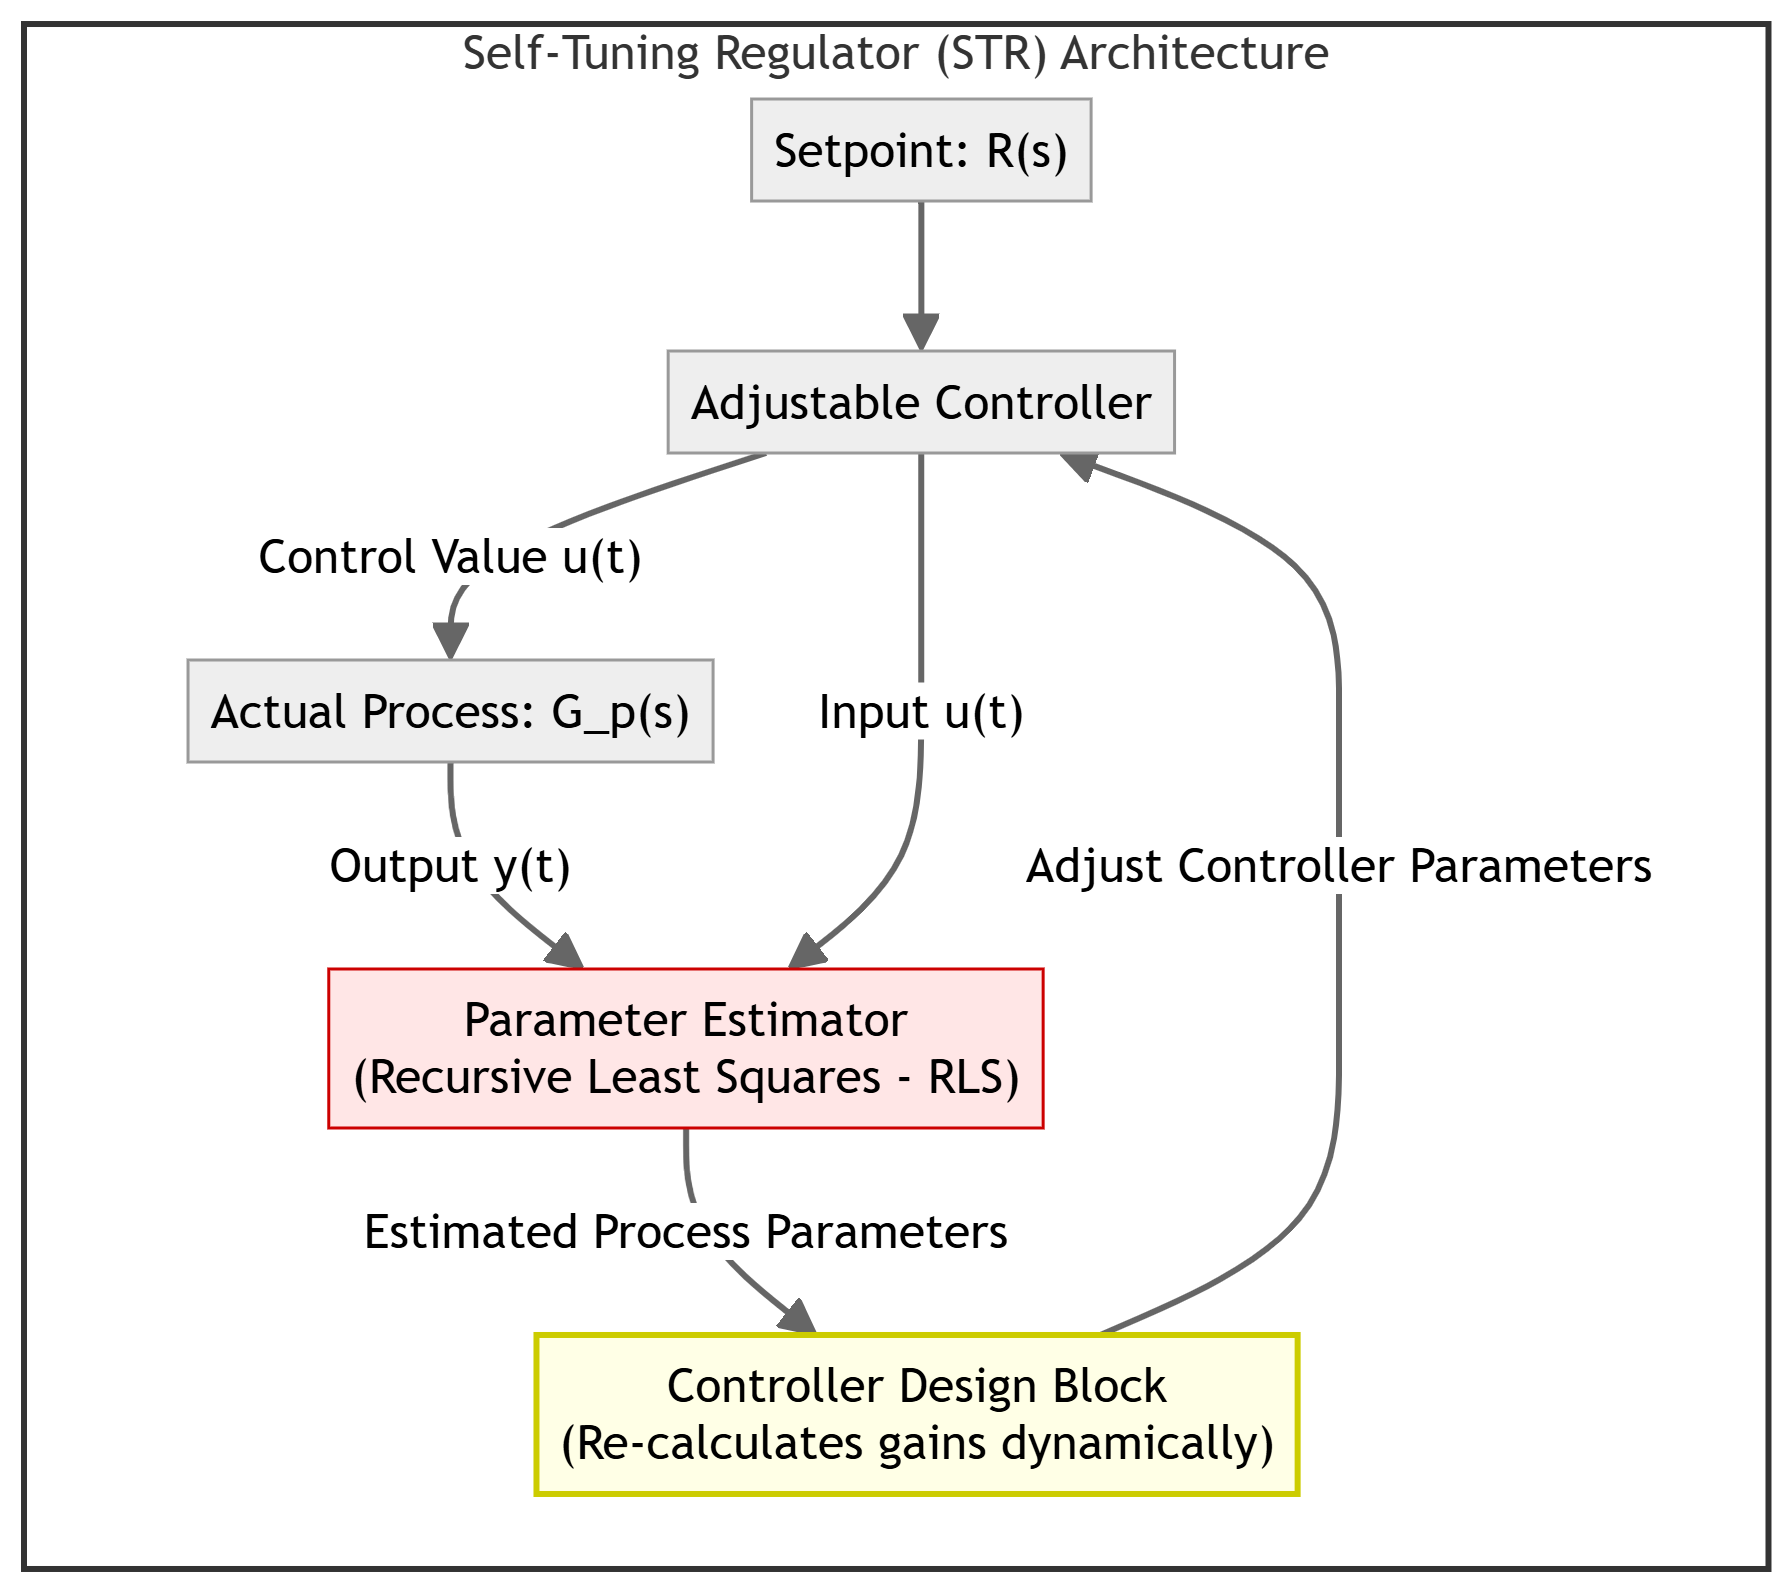
\includegraphics[width=0.75\textwidth,height=0.32\textheight,keepaspectratio]{../Images/chapter_04/str_block.png}
\caption{Self-Tuning Regulator (STR)}
\end{figure}


\subsection{2. Internal Model Control (IMC)}
\textbf{Internal Model Control (IMC)} is a model-based control strategy where an explicit mathematical model of the process is run in parallel with the physical process.

\begin{figure}[H]
\centering
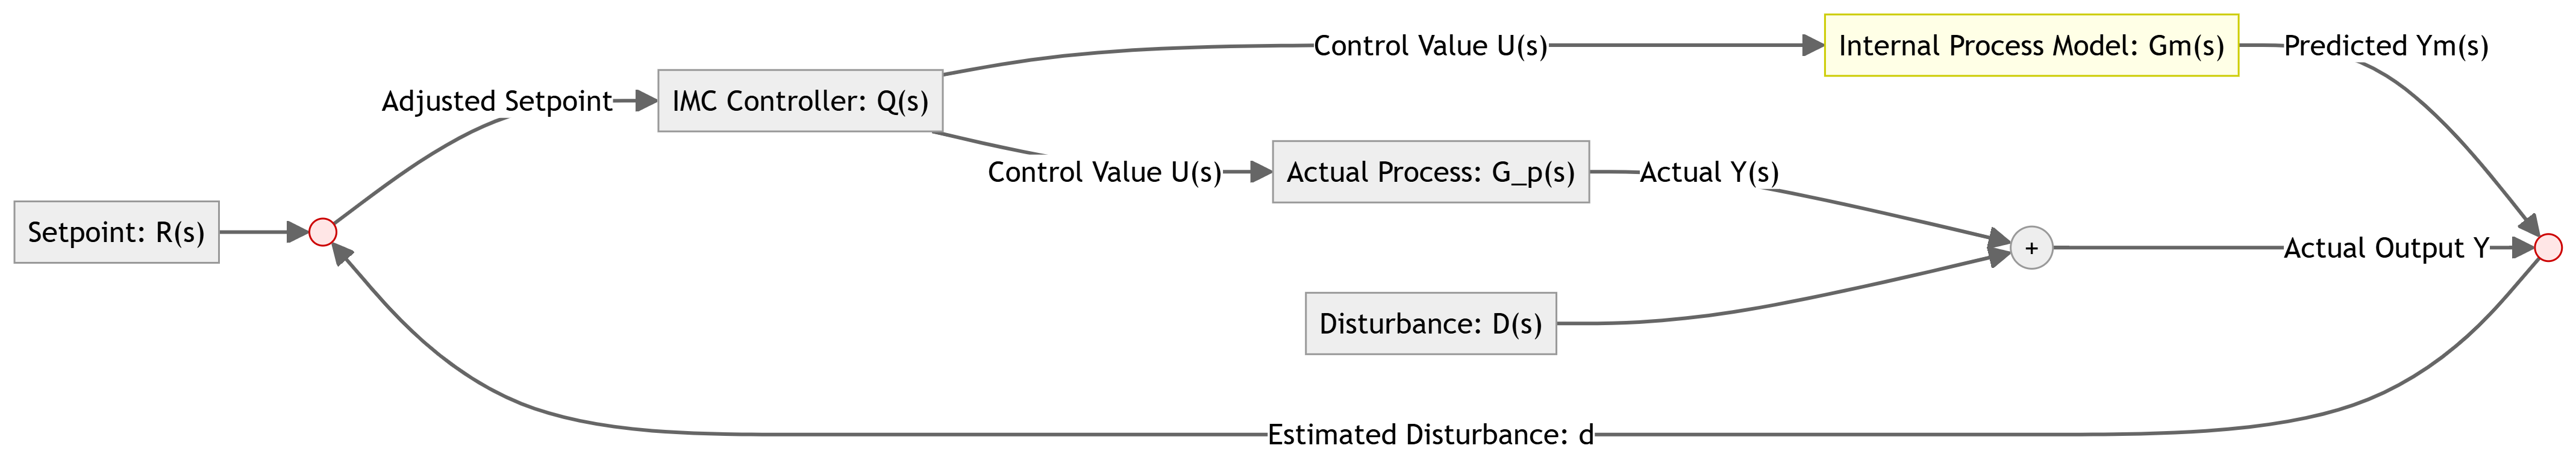
\includegraphics[width=0.75\textwidth,height=0.32\textheight,keepaspectratio]{../Images/chapter_04/imc_block.png}
\caption{Internal Model Control (IMC) Block Diagram}
\end{figure}

\subsubsection{A. Working Principle}
\begin{itemize}
  \item The controller output is sent to both the physical process $G_p(s)$ and the process model $\tilde{G}_p(s)$.
  \item The predicted model output ($\tilde{Y}$) is subtracted from the actual measured process output ($Y$). This difference represents the unmodeled disturbances and model mismatch ($d = Y - \tilde{Y}$).
  \item This difference is fed back to the setpoint summing junction.
  \item \textbf{Advantage:} If the model matches the process exactly ($\tilde{G}_p = G_p$) and there are no disturbances, the feedback signal is zero, and the control loop operates in an open-loop fashion, improving system stability. The IMC structure also simplifies the design of controllers for processes with dead time.
\end{itemize}
